\documentclass{beamer}
\usepackage[utf8]{inputenc}
\usepackage[brazil]{babel}

\usetheme{Warsaw}
\bibliographystyle{abnt-alf}

\institute{Universidade Tuiuti do Paraná}
\author{Bogdano Arendartchuk}
\title{Avaliação de técnicas de predição de comportamento de máquinas
virtuais para a otimização de uso de parque computacional}
\date{\today}

\setbeamertemplate{footline}{
  \leavevmode%
  \hbox{%
  \begin{beamercolorbox}[wd=\paperwidth,ht=5.25ex,dp=1ex,right]{date in head/foot}%
    \insertframenumber{} \hspace*{2ex}
  \end{beamercolorbox}}%
  \vskip0pt%
}

\begin{document}

\frame{\titlepage}

\section{Contextualização}
\begin{frame}
\begin{block}{Virtualização}
Consiste na execução simulada de cada instrução de uma determinada
arquitetura bem como a emulação de seu hardware original, de maneira a
permitir que qualquer sistema operacional compatível possa também executar
neste ambiente.\cite{goldberg1974survey}
\end{block}
\end{frame}

%% \begin{columns}[c]
%% \column{1.5in}
%% \center
%% \includegraphics[width=4cm]{dutra2009-arq-virtualizacao.png}
%% \column{1.5in}
%% Foo bar baz.
%% \end{columns}
\begin{frame}{Arquitetura clássica}
\begin{figure}
\centering
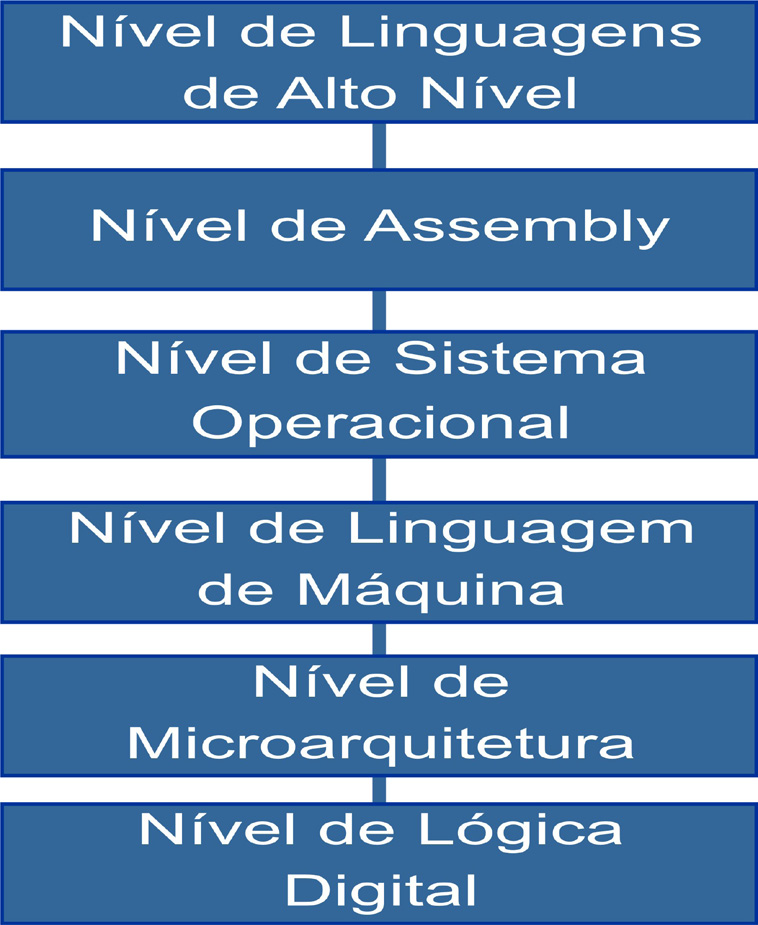
\includegraphics[height=5cm]{img-dutra2009-clas.png}
\end{figure}
\tiny{Fonte: \cite{dutra2009a}}
\end{frame}

\begin{frame}{Arquitetura de virtualização}
\begin{figure}
\centering
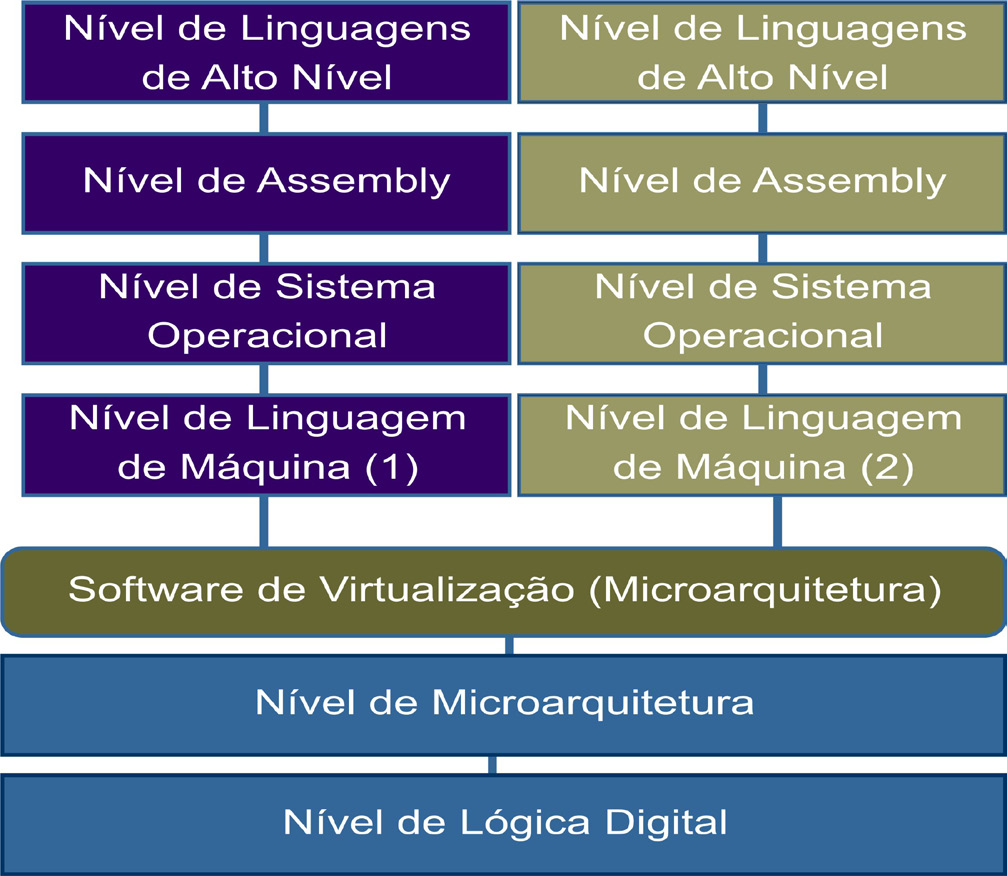
\includegraphics[height=5cm]{img-dutra2009-virt.png}
\end{figure}
\tiny{Fonte: \cite{dutra2009a}}
\end{frame}

\begin{frame}{Monitores de Máquinas Virtuais}
% talvez citar que estão cada vez mais focados em cloud computing, blabla
\begin{itemize}
  \item VMware
  \item Xen
  \item Virtualbox
  \item QEMU
  \item KVM
\end{itemize}
\end{frame}

\begin{frame}{\emph{libvirt}}
\begin{itemize}
  \item abstrai acesso aos MMV
% opensaucer
% etc
\end{itemize}
\end{frame}

\begin{frame}{Ambiente de virtualização I}
\begin{figure}
\centering
% imagem ilustrando um ambiente com um host e várias máquinas virtuais,
% descrição das situações em que é possível executar "migração de máquinas
% virtuais"
%
% talvez até poderia também já descrever como é um ambiente completo
%
\includegraphics[height=5cm]{}
\end{figure}
\end{frame}

\section{Metodologia}

\begin{frame}{Antes de tudo}
\begin{block}{}
O título \textbf{Avaliação de técnicas de predição de comportamento de máquinas
virtuais para a otimização de uso de parque computacional} é inadequado.
\end{block}
\end{frame}

\begin{frame}{Problemas conhecidos}
\begin{itemize}
  \item O título \textbf{Avaliação de técnicas de predição de comportamento
        de máquinas virtuais para a otimização de uso de parque computacional} é
        inadequado.
  \item 
\end{itemize}
\end{frame}

\section{Conclusões}
\frame{\frametitle{Conclusões}}
\frame{\frametitle{Referências}
  \bibliography{biblio}}
\frame{\frametitle{Dúvidas?} \centering{Dúvidas?}}

\end{document}
